% Options for packages loaded elsewhere
\PassOptionsToPackage{unicode}{hyperref}
\PassOptionsToPackage{hyphens}{url}
%
\documentclass[
]{book}
\usepackage{lmodern}
\usepackage{amssymb,amsmath}
\usepackage{ifxetex,ifluatex}
\ifnum 0\ifxetex 1\fi\ifluatex 1\fi=0 % if pdftex
  \usepackage[T1]{fontenc}
  \usepackage[utf8]{inputenc}
  \usepackage{textcomp} % provide euro and other symbols
\else % if luatex or xetex
  \usepackage{unicode-math}
  \defaultfontfeatures{Scale=MatchLowercase}
  \defaultfontfeatures[\rmfamily]{Ligatures=TeX,Scale=1}
\fi
% Use upquote if available, for straight quotes in verbatim environments
\IfFileExists{upquote.sty}{\usepackage{upquote}}{}
\IfFileExists{microtype.sty}{% use microtype if available
  \usepackage[]{microtype}
  \UseMicrotypeSet[protrusion]{basicmath} % disable protrusion for tt fonts
}{}
\makeatletter
\@ifundefined{KOMAClassName}{% if non-KOMA class
  \IfFileExists{parskip.sty}{%
    \usepackage{parskip}
  }{% else
    \setlength{\parindent}{0pt}
    \setlength{\parskip}{6pt plus 2pt minus 1pt}}
}{% if KOMA class
  \KOMAoptions{parskip=half}}
\makeatother
\usepackage{xcolor}
\IfFileExists{xurl.sty}{\usepackage{xurl}}{} % add URL line breaks if available
\IfFileExists{bookmark.sty}{\usepackage{bookmark}}{\usepackage{hyperref}}
\hypersetup{
  pdftitle={Project Primer},
  pdfauthor={Dan Spalla},
  hidelinks,
  pdfcreator={LaTeX via pandoc}}
\urlstyle{same} % disable monospaced font for URLs
\usepackage{longtable,booktabs}
% Correct order of tables after \paragraph or \subparagraph
\usepackage{etoolbox}
\makeatletter
\patchcmd\longtable{\par}{\if@noskipsec\mbox{}\fi\par}{}{}
\makeatother
% Allow footnotes in longtable head/foot
\IfFileExists{footnotehyper.sty}{\usepackage{footnotehyper}}{\usepackage{footnote}}
\makesavenoteenv{longtable}
\usepackage{graphicx}
\makeatletter
\def\maxwidth{\ifdim\Gin@nat@width>\linewidth\linewidth\else\Gin@nat@width\fi}
\def\maxheight{\ifdim\Gin@nat@height>\textheight\textheight\else\Gin@nat@height\fi}
\makeatother
% Scale images if necessary, so that they will not overflow the page
% margins by default, and it is still possible to overwrite the defaults
% using explicit options in \includegraphics[width, height, ...]{}
\setkeys{Gin}{width=\maxwidth,height=\maxheight,keepaspectratio}
% Set default figure placement to htbp
\makeatletter
\def\fps@figure{htbp}
\makeatother
\setlength{\emergencystretch}{3em} % prevent overfull lines
\providecommand{\tightlist}{%
  \setlength{\itemsep}{0pt}\setlength{\parskip}{0pt}}
\setcounter{secnumdepth}{5}
\usepackage{booktabs}
\usepackage[]{natbib}
\bibliographystyle{apalike}

\title{Project Primer}
\author{Dan Spalla}
\date{2020-06-30}

\begin{document}
\maketitle

{
\setcounter{tocdepth}{1}
\tableofcontents
}
\hypertarget{preface}{%
\chapter*{Preface}\label{preface}}
\addcontentsline{toc}{chapter}{Preface}

This documentation is a primer for the COVID-19 DCTT BCS-2032203 project. It covers an introduction to Git, using Git in RStudio, an introduction to RMarkdown, the project repository, and project helper scripts.

This documentation assumes an introductory understanding of the R programming language and RStudio. It also assumes zero knowledge of Git, using Git in RStudio, and RMarkdown; consequently, some explanations may be structured or phrased in a way that are conducive to understanding but not perfectly accurate.

\hypertarget{git-introduction}{%
\chapter{Git Introduction}\label{git-introduction}}

\hypertarget{what-is-git}{%
\section{What is Git?}\label{what-is-git}}

Git is a distributed version control system that was developed by Linus Torvalds for working on the Linux kernel. Despite its original use case, it is used for many software projects. It has become a popular choice for version control systems and becomes a powerful tool once the basics are learned.

Users traditionally interface with Git through a Unix shell, or commandline environment, but there are several graphical or GUI options for interfacing with the tool. More information about this can be found in the Appendix section of this documentation.

Git, and version control systems more generally, enable users to store different versions of files and keep track of changes between those versions. Git helps users document a history of changes, including mistakes, to their projects and enables them to switch to any past version. The result is essentially a list of different versions of a project that represent its state during a given time.

\hypertarget{what-is-a-repository}{%
\section{What is a Repository?}\label{what-is-a-repository}}

A Git repository is a directory, or folder, where version tracking and history has been initialized. One can check if version tracking is initialized in a directory by looking for a hidden ``.git'' subdirectory (you may have to enable a, ``show hidden files'' feature in your file manager if you wish to do this). This hidden directory stores metadata about a project, metadata of the files in that project, and the detailed history of that project. Note that the actual project files reside in the directory that contains the hidden ``.git'' directory, not the ``.git'' directory itself.

A repository is an entity that is local in nature, meaning it resides on your machine and you treat it the same way you would any other file. As a result, any changes you make are yours and you must deliberately choose to share those changes if you want others to see them.

\hypertarget{what-is-a-commit}{%
\section{What Is A Commit?}\label{what-is-a-commit}}

A commit is a change to a repository and you do this when you implement a change to your project. This change can be as simple as the addition of a new file to your project or as complex as a series of changes across multiple files. A user ``commits'' to a repository when they want to store a new version of a project. When this is done, they now have a distinct version of the project that they can go back to and view the changes from one version to another.

Generally, commits should contain a change that is singular in purpose. If two separate parts of a project were to be changed, they should be ``committed'' to the repository separately. A commit represents a point in time, a specific version of your project, and if two changes representing separate parts of a project were to end up in the same commit, then it would make the history of your project confusing or not clear. It is desirable to be able to understand the evolution of a project as changes are made and this becomes more difficult if changes are not distinct.

A commit will have a message associated with it. This message should describe why changes were made and what purpose these changes fulfill. Each commit will have a log of what aspects of your project have changed and a commit message should also briefly describe what changes were made if they are not self-explanatory.

For the sake of argument, let's say you change a readme file to include a link to a funding page for your project. The following is an example of a poor commit message.

\begin{quote}
Changed the readme.
\end{quote}

A better message would be:

\begin{quote}
Added a link to the funding page.
\end{quote}

An even better message would be:

\begin{quote}
Added a link to the funding page in the reference section of the readme. Those who want to fund the project no longer have to email asking how to support it.
\end{quote}

\hypertarget{understanding-distributed}{%
\section{Understanding Distributed}\label{understanding-distributed}}

As was stated previously, Git is a distributed version control system which means that every repository, including ones on your local machine, do not require some centralized service to function.

When you share changes with others, you are simply merging histories or syncing changes rather than performing some sort of special transaction with a centralized service. It is important to have a conceptual understanding of this because this is how you use Git when working on a project. You make and commit changes locally, then you can share those changes with the rest of the world. You cannot share changes with the rest of the world if you have not committed those changes locally.

\hypertarget{push}{%
\section{Push}\label{push}}

The act of ``push'', or ``pushing'', is when changes are uploaded to remote locations. Once a change is made and committed to your local repository, you can then send a copy of your changes to a remote location (push). This remote location is simply housing another copy of that repository. Anyone with the proper permissions can push to a remote repository so that someone else can download (pull) their changes.

\hypertarget{pull}{%
\section{Pull}\label{pull}}

The act of ``pull'', or ``pulling'', is when changes are downloaded from remote locations. If someone pushes a change into a remote repository, you can download (pull) that change and sync it with your local repository. Anyone can pull changes from a remote repository and sync it with their local version. This is also how repositories are initially downloaded if they are not present on your machine.

\hypertarget{the-log}{%
\section{The Log}\label{the-log}}

Each Git repository has its own history that details which files have changed, who changed them, and their stated reasons for changing them. This can be viewed by using the log functionality of Git. The log will give you an overview of each project change by showing all the aforementioned information as well as detailing the exact changes. This can be used to track project changes and understand its history.

\hypertarget{using-git-in-rstudio}{%
\chapter{Using Git in Rstudio}\label{using-git-in-rstudio}}

\hypertarget{initializing-a-repository-for-a-new-project}{%
\section{Initializing a Repository For a New Project}\label{initializing-a-repository-for-a-new-project}}

If you haven't yet created a new project in RStudio, you can check the ``Create a git repository'' box in the new project wizard to automatically create one for you.

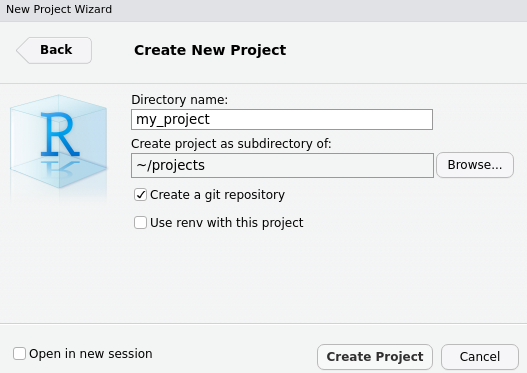
\includegraphics{images/02-newgit_1.png}

If you already have an existing project but wish to initialize a Git repository for it, its quite simple.

\begin{enumerate}
\def\labelenumi{\arabic{enumi}.}
\tightlist
\item
  Select ``Tools'' from the toolbar, ``Version Control'', and click on ``Project Setup\ldots{}''
\end{enumerate}

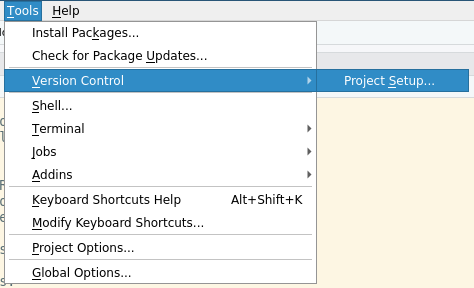
\includegraphics{images/02-newgit_2.png}

\begin{enumerate}
\def\labelenumi{\arabic{enumi}.}
\setcounter{enumi}{1}
\tightlist
\item
  Select ``Git'' from the dropdown box
\end{enumerate}

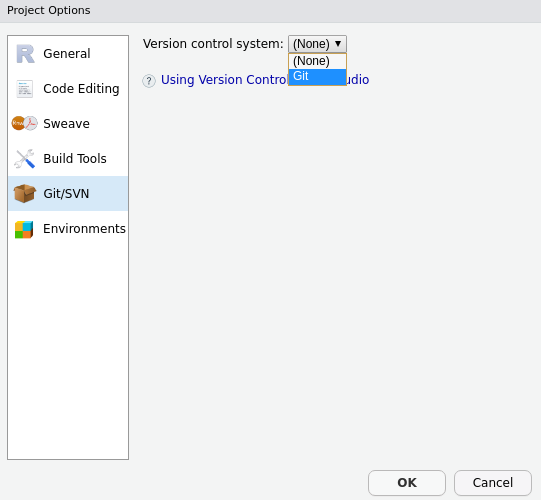
\includegraphics{images/02-newgit_3.png}

\begin{enumerate}
\def\labelenumi{\arabic{enumi}.}
\setcounter{enumi}{2}
\tightlist
\item
  Confirm that you want to create a new Git repository
\end{enumerate}


\includegraphics{images/02-newgit_4.png}

\begin{enumerate}
\def\labelenumi{\arabic{enumi}.}
\setcounter{enumi}{3}
\tightlist
\item
  It may ask you to restart RStudio; restart RStudio
\end{enumerate}


\includegraphics{images/02-newgit_5.png}

\begin{enumerate}
\def\labelenumi{\arabic{enumi}.}
\setcounter{enumi}{4}
\tightlist
\item
  The Git tab will appear on the top-right window and show the status of your new repository
\end{enumerate}

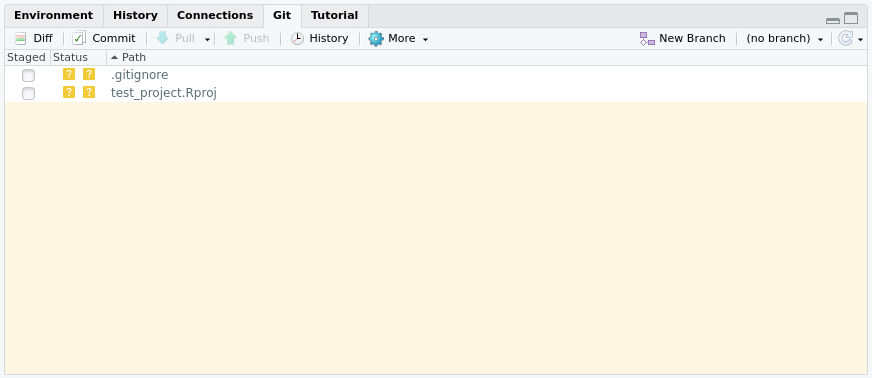
\includegraphics{images/02-newgit_6.png}

\hypertarget{creating-a-project-from-a-git-repository}{%
\section{Creating a Project From a Git Repository}\label{creating-a-project-from-a-git-repository}}

Creating a new RStudio project from a Git repository, such as one hosted on GitHub, is quite simple.

\begin{enumerate}
\def\labelenumi{\arabic{enumi}.}
\tightlist
\item
  Create a new project
\item
  Select ``Version Control''
\end{enumerate}

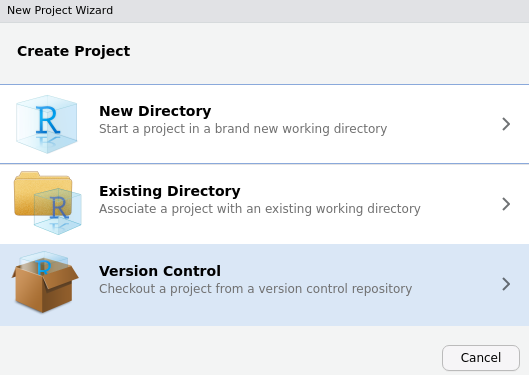
\includegraphics{images/02-newprojectgit_1.png}

\begin{enumerate}
\def\labelenumi{\arabic{enumi}.}
\setcounter{enumi}{2}
\tightlist
\item
  Select ``Git''
\end{enumerate}

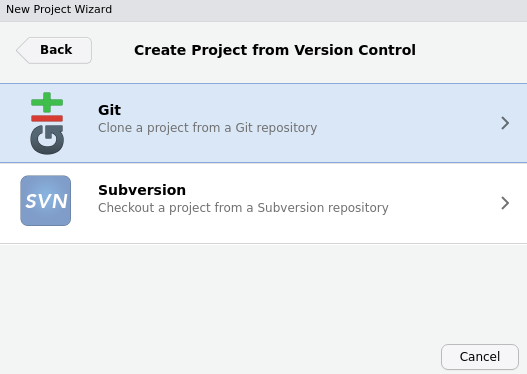
\includegraphics{images/02-newprojectgit_2.png}

\begin{enumerate}
\def\labelenumi{\arabic{enumi}.}
\setcounter{enumi}{3}
\tightlist
\item
  Enter the repository URL, give the project a name, and select the directory where project files shall reside
\end{enumerate}

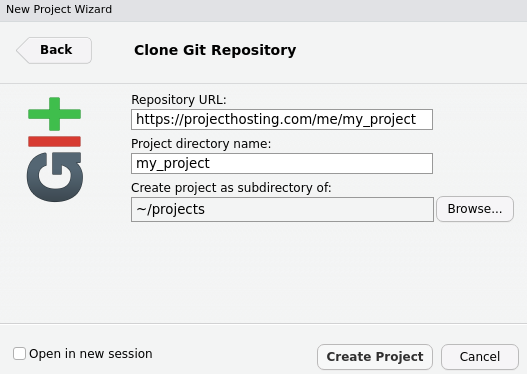
\includegraphics{images/02-newprojectgit_3.png}

\hypertarget{making-changes-and-committing}{%
\section{Making Changes and Committing}\label{making-changes-and-committing}}

To make changes to files in a git repository, modify them you would any other file. When you are ready to commit your changes, do the following.

\begin{enumerate}
\def\labelenumi{\arabic{enumi}.}
\tightlist
\item
  Hit the commit button under the Git tab and a new window will appear
\end{enumerate}


\includegraphics{images/02-commit_1.png}

\begin{enumerate}
\def\labelenumi{\arabic{enumi}.}
\setcounter{enumi}{1}
\tightlist
\item
  Select, stage, the changed files that you wish to add and commit
\end{enumerate}

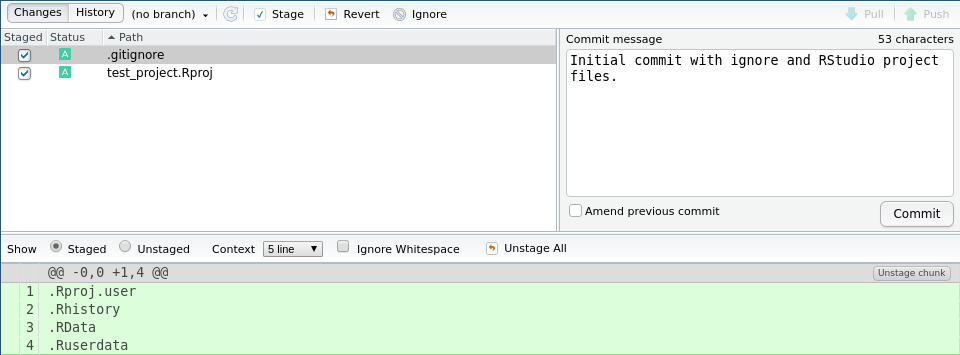
\includegraphics{images/02-commit_2.png}

\begin{enumerate}
\def\labelenumi{\arabic{enumi}.}
\setcounter{enumi}{2}
\tightlist
\item
  Write a commit message that succinctly describes the ``what'' and ``why'' of your changes and hit the commit button. A status window will show whether or not it was successful
\end{enumerate}

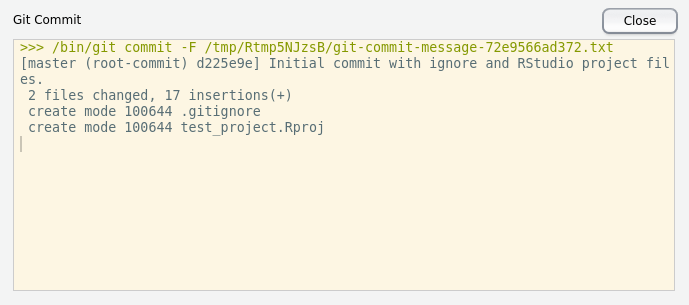
\includegraphics{images/02-commit_3.png}

\hypertarget{sharing-those-changes-push}{%
\section{Sharing Those Changes, Push}\label{sharing-those-changes-push}}

When you are ready to share your changes with the rest of the world, press the push button under the Git tab or on the commit window.


\includegraphics{images/02-commit_1.png}

A status window will appear and show its success.

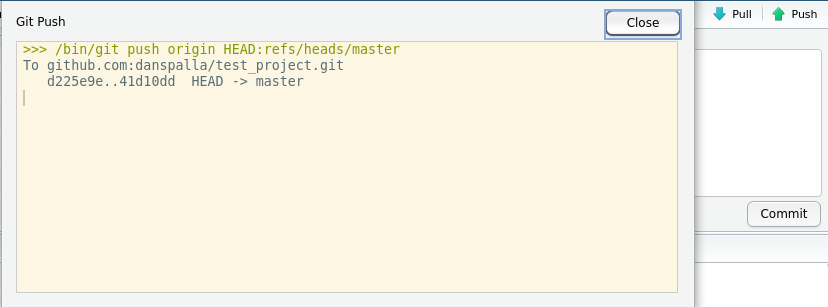
\includegraphics{images/02-push_1.png}

\hypertarget{getting-changes-from-others-pull}{%
\section{Getting Changes From Others, Pull}\label{getting-changes-from-others-pull}}

To receive updates that others have pushed, hit the pull button under the Git tab.


\includegraphics{images/02-commit_1.png}

A status window will appear and show its success.

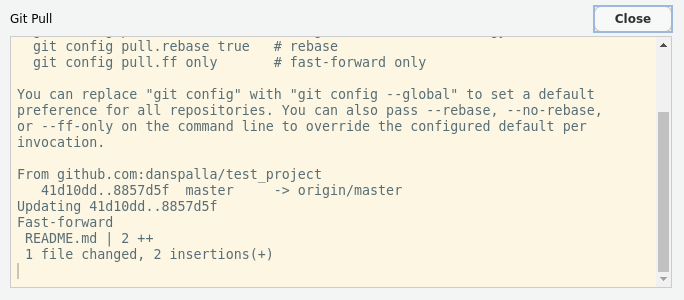
\includegraphics{images/02-pull_1.png}

\hypertarget{viewing-the-log}{%
\section{Viewing the Log}\label{viewing-the-log}}

You can view the git log for a repository by clicking the history button.


\includegraphics{images/02-commit_1.png}

You can click on each commit, read each commit changes, and see what files in the project were changed for that commit.

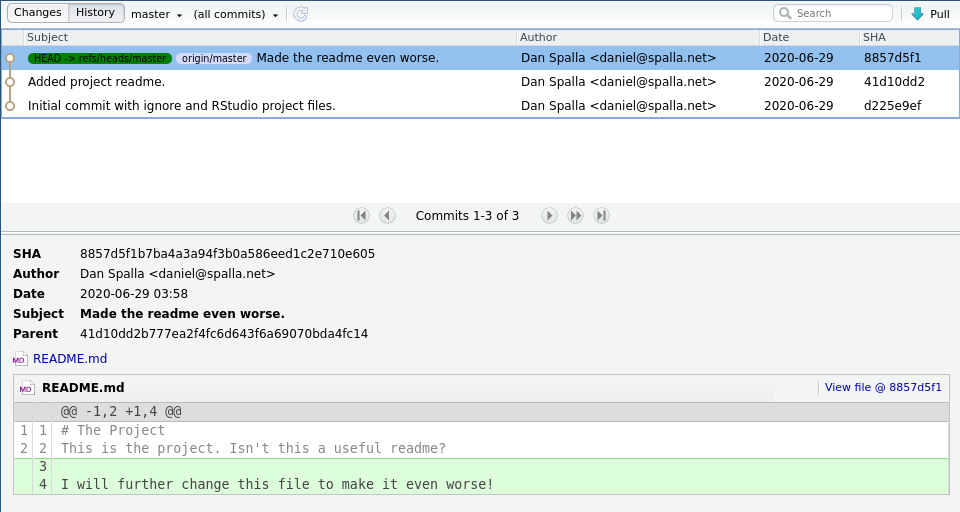
\includegraphics{images/02-log_1.png}

\hypertarget{rmarkdown-introduction}{%
\chapter{RMarkdown Introduction}\label{rmarkdown-introduction}}

\hypertarget{what-is-markdown}{%
\section{What is Markdown?}\label{what-is-markdown}}

Markdown is a markup language that enables a user to type a certain syntax and always generate the same output documents. There are no hidden characters or special formatting, that you would inevitably encounter using a word processor, which could cause unwanted changes to appearance of a document. Please see the, ``Markdown Introductory Tutorial'' in the appendix for a basic interactive tutorial.

\hypertarget{what-is-rmarkdown}{%
\section{What is RMarkdown?}\label{what-is-rmarkdown}}

RMarkdown is an extension of the Markdown markup language that allows the user to embed R code in Markdown documents. A markup language is a simple set of syntax that when written will always produce the same output document (as opposed to WYSIWYG editors). RMarkdown extends this by embedding R code into the documents, showcasing the source code, a R script's output, and any figures generated by the R script.

Example of source code and output below.

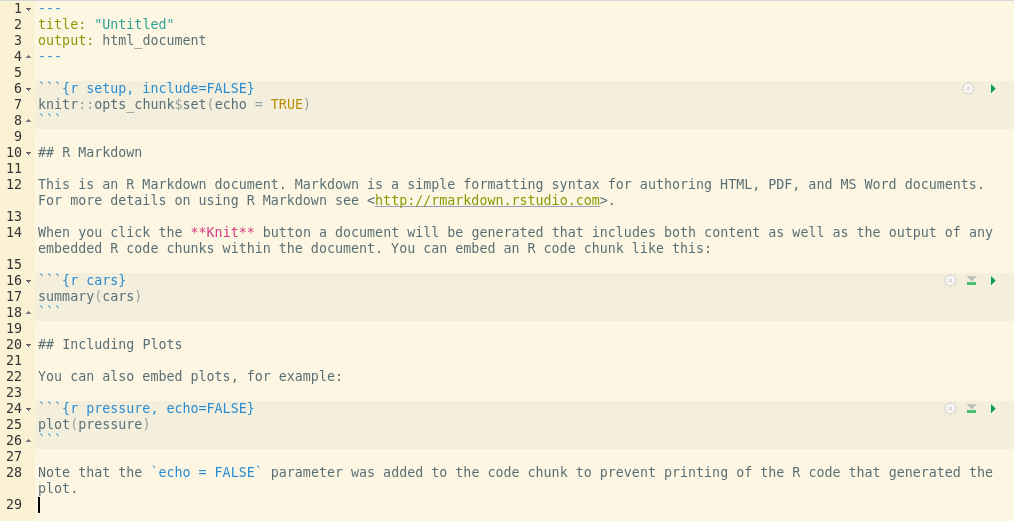
\includegraphics{images/03-rmarkdown_1.png}

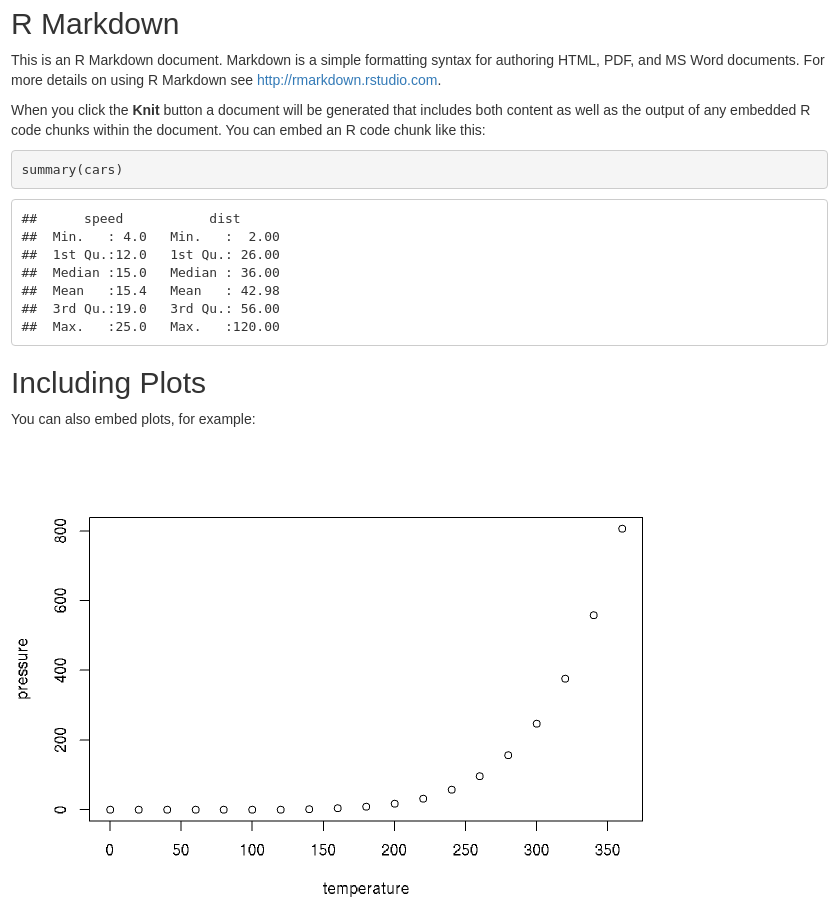
\includegraphics{images/03-rmarkdown_2.png}

\hypertarget{r-code-in-rmarkdown}{%
\section{R Code in RMarkdown}\label{r-code-in-rmarkdown}}

There are two ways to include R code in an RMarkdown document. The first is to simply inline the code in the document itself and compile the document. The second way is to load the code from a file instead of inlining in the document. Loading the code from a file provides a nice separation between the data processing and data presentation of a R script. The second method should be used if the R code is lengthy, complicated, or needs to be worked on independent of successful RMarkdown document compilation.

To load a R script from a file, simply add ``code = readlines(''location\_to\_file``)'' and specify the path to the file.

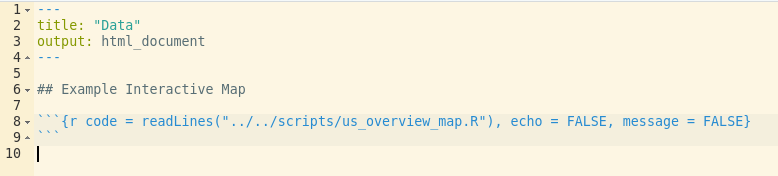
\includegraphics{images/04-example2_3.png}

\hypertarget{contribution-to-project}{%
\chapter{Contribution to Project}\label{contribution-to-project}}

\hypertarget{project-repository}{%
\section{Project Repository}\label{project-repository}}

The project repository can be found at \href{https://github.com/Peter-Kedron/COVID-19-Digital-Contact-Tracing-and-Geospatial-Technologies-and-Privacy}{GitHub}. The repository provides the website, website source code, geodatabase, and helper scripts.

\hypertarget{overview-of-project-technologies}{%
\section{Overview of Project Technologies}\label{overview-of-project-technologies}}

The project makes use of a number of technologies.

\begin{itemize}
\tightlist
\item
  R: used for scripts that help manage website content updates, interactive map, and analysis.
\item
  RMarkdown: used to create website pages and embed R code
\item
  RStudio: (optional), used to facilitate easy project contribution and management
\end{itemize}

\hypertarget{repository-directory-hierarchy}{%
\section{Repository Directory Hierarchy}\label{repository-directory-hierarchy}}

The repository uses the following directory hierarchy:

\begin{itemize}
\tightlist
\item
  /website: Folder where the website source code is stored; new content for the website is created and added here.
\item
  /docs: ``Mount point'' for GitHub pages; the project can be configured to serve the website from this folder (GitHub provides no flexibility on this), requiring no further intervention from team members.
\item
  /data: Folder where any data files are stored for use in R scripts or RMarkdown files.
\item
  /scripts: Folder where any R scripts, or other software scripts/tools, are stored. Ex: Helper scripts for building and local previewing of the website are stored here.
\end{itemize}

\hypertarget{how-to-use-the-helper-scripts}{%
\section{How To Use The Helper Scripts}\label{how-to-use-the-helper-scripts}}

The following helper scripts are currently available for use in the ``/scripts'' directory.

\begin{itemize}
\tightlist
\item
  ``project\_install\_dependencies.R'': This script installs all the dependencies needed on the project. This should be used when the project has been pulled for the first time.
\item
  ``website\_preview.R'': This script will automatically build the website locally and launch a local web server that can be used to preview the site. This mode will continuously check website files for update and automatically rebuild the site so that changes can be easily previewed.
\item
  ``website\_build.R'': This script builds the website without providing a preview to the user.
\end{itemize}

\hypertarget{getting-started-with-contribution}{%
\section{Getting Started With Contribution}\label{getting-started-with-contribution}}

To get started contributing to the project, use the following steps.

Using RStudio:

\begin{enumerate}
\def\labelenumi{\arabic{enumi}.}
\tightlist
\item
  Open RStudio
\item
  Create a new project, select the version control option, select Git as the version control system, and enter the GitHub repository URL
\item
  Wait for RStudio to automatically pull the latest project files from GitHub
\item
  Navigate to the scripts folder and run the, ``project\_install\_dependencies.R'' script; this will install all dependencies and may take some time.
\end{enumerate}

\hypertarget{contribution-example-1}{%
\section{Contribution Example 1}\label{contribution-example-1}}

Scenario: Update the website title to better reflect the project.

\begin{enumerate}
\def\labelenumi{\arabic{enumi}.}
\tightlist
\item
  Navigate to the ``/website'' directory
\item
  Open the, ``config.toml'' file
\item
  Change the line that says, `title = ``COVID-19 DCTT''\,' and change it to, `title = ``COVID-19 DCTT!''\,'; save the file
\end{enumerate}

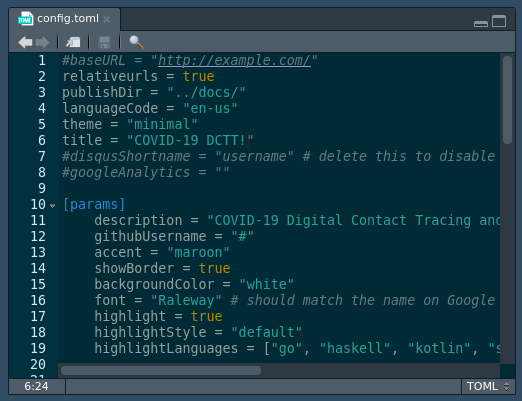
\includegraphics{images/04-example1_1.png}

\begin{enumerate}
\def\labelenumi{\arabic{enumi}.}
\setcounter{enumi}{3}
\tightlist
\item
  Navigate to the ``/scripts'' directory and run the, ``website\_preview.R'' script to preview the website
\item
  Notice that there are changes in the ``/website'' directory and the ``/docs'' directory in the Git tab
\end{enumerate}

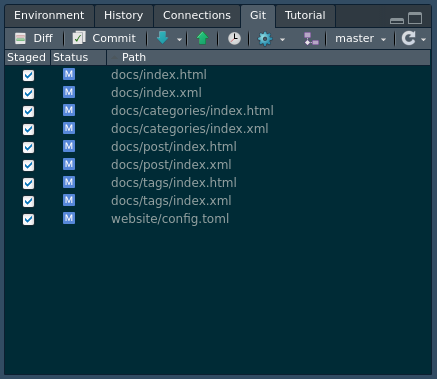
\includegraphics{images/04-example1_2.png}

\begin{enumerate}
\def\labelenumi{\arabic{enumi}.}
\setcounter{enumi}{5}
\tightlist
\item
  Commit changes to your local repository stating the change
\end{enumerate}

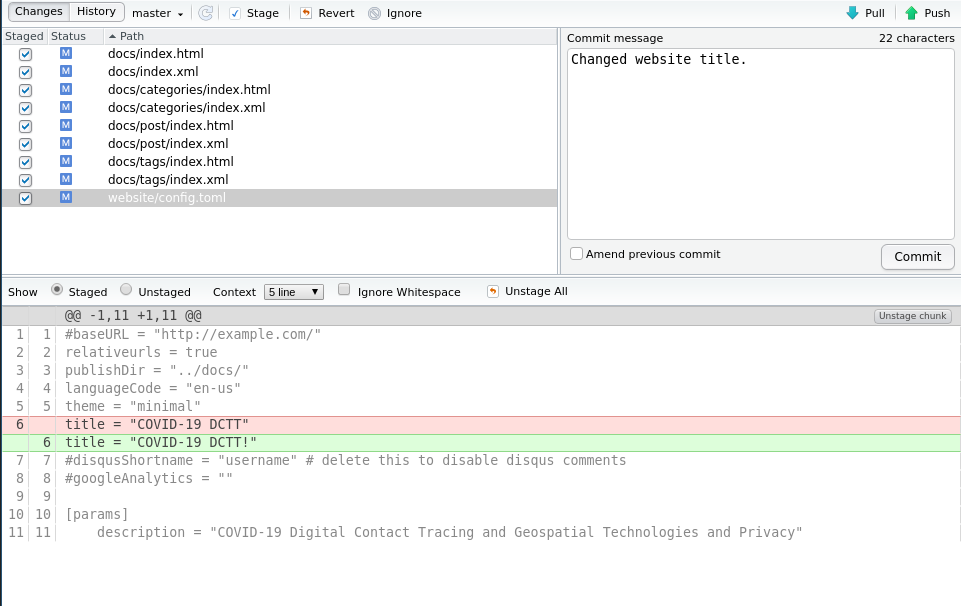
\includegraphics{images/04-example1_3.png}

\begin{enumerate}
\def\labelenumi{\arabic{enumi}.}
\setcounter{enumi}{6}
\tightlist
\item
  Push your changes to the GitHub repository to share the changes with the team.
\end{enumerate}

\hypertarget{contribution-example-2}{%
\section{Contribution Example 2}\label{contribution-example-2}}

Scenario: Create an interactive overview map for the US to show which states are using digital contact tracing and which states are not; include the technology used and application name if available.

\begin{enumerate}
\def\labelenumi{\arabic{enumi}.}
\tightlist
\item
  Obtain the state data on DCTT, put the file in the ``/data'' directory
\end{enumerate}

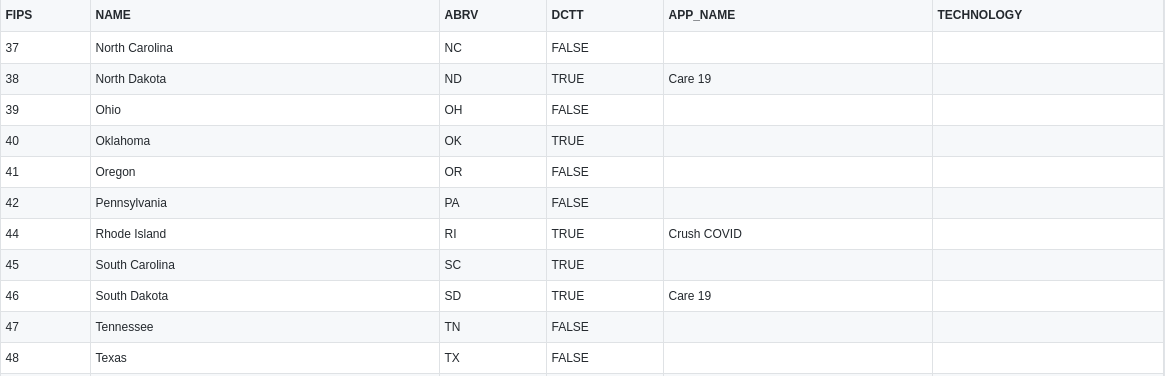
\includegraphics{images/04-example2_1.png}
2. Place the shapefile that will be used in the ``/data'' folder as well
3. Write an R script to generate the interactive map and place it in the ``/scripts'' directory

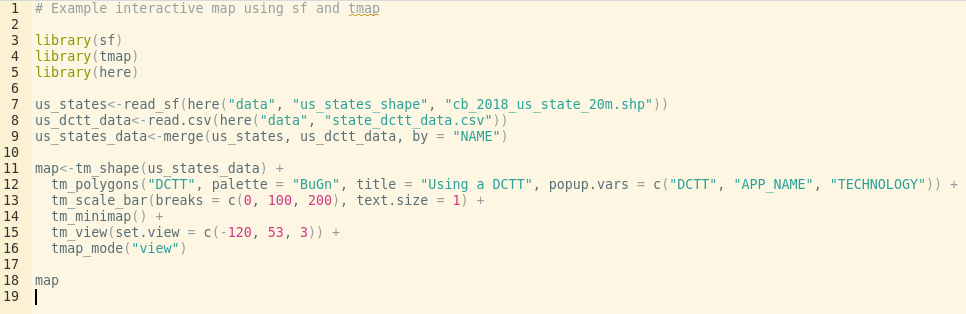
\includegraphics{images/04-example2_2.png}
4. Modify the RMarkdown document on the page we want to display the map, and add the location of the script

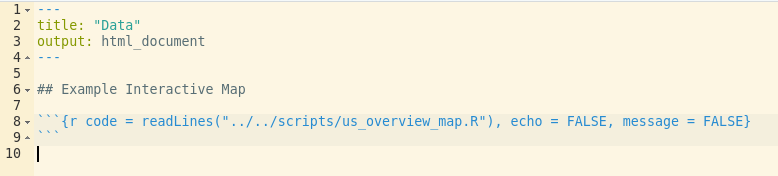
\includegraphics{images/04-example2_3.png}
5. Run the ``website\_preview.R'' from the ``/scripts'' directory to preview the map locally

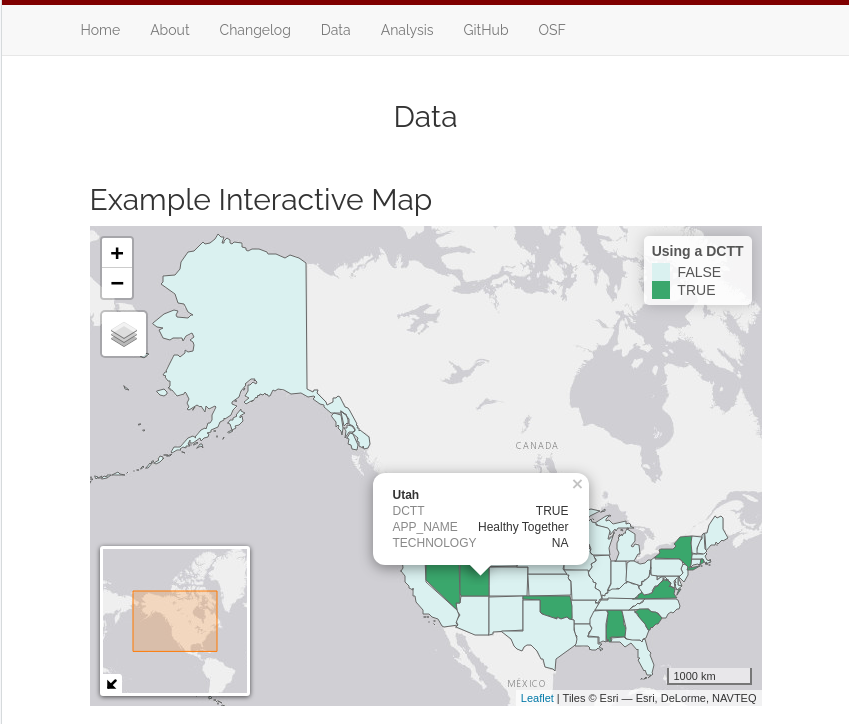
\includegraphics{images/04-example2_4.png}
6. Commit the changes to the ``/data'', ``/scripts'', ``website'', and ``/docs'' directories to your local repository
7. Push the changes to the GitHub repository to update the website and share the interactive map with the team

\hypertarget{creating-a-new-page}{%
\section{Creating a New Page}\label{creating-a-new-page}}

Creating a new page for the website requires a number of changes across the website source files.

\begin{enumerate}
\def\labelenumi{\arabic{enumi}.}
\tightlist
\item
  Create a new RMarkdown file from the ``File -\textgreater{} New File'' menu.
\end{enumerate}

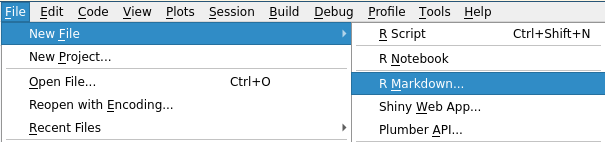
\includegraphics{images/04-newpage_1.png}

\begin{enumerate}
\def\labelenumi{\arabic{enumi}.}
\setcounter{enumi}{1}
\tightlist
\item
  Give the file an appropriate title and make sure HTML is the output format
\end{enumerate}

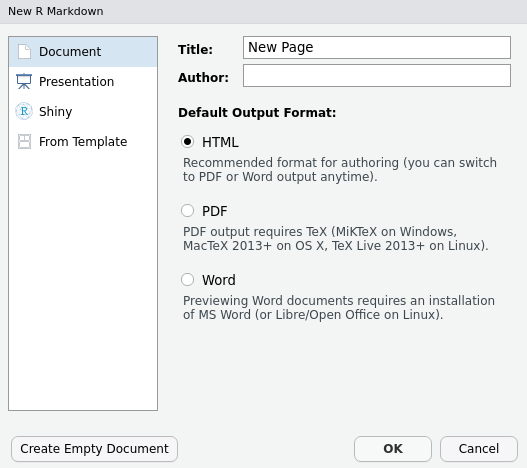
\includegraphics{images/04-newpage_2.png}

\begin{enumerate}
\def\labelenumi{\arabic{enumi}.}
\setcounter{enumi}{2}
\tightlist
\item
  Save the file in the content directory: ``/website/content/''
\end{enumerate}

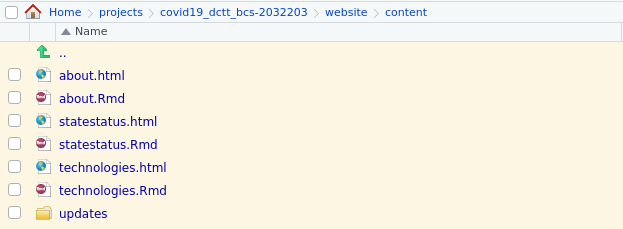
\includegraphics{images/04-newpage_4.png}

\begin{enumerate}
\def\labelenumi{\arabic{enumi}.}
\setcounter{enumi}{3}
\tightlist
\item
  Open the ``config.toml'' configuration file located in ``/website/''
\end{enumerate}

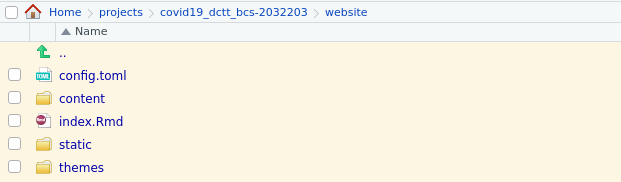
\includegraphics{images/04-newpage_3.png}

\begin{enumerate}
\def\labelenumi{\arabic{enumi}.}
\setcounter{enumi}{4}
\tightlist
\item
  Add the following entry to the configuration file to add the page to the navigation bar
\end{enumerate}

\begin{quote}
{[}{[}menu.main{]}{]}

\begin{quote}
url = ``/page\_file\_name/''

name = ``Pretty Page Name''

weight = 5
\end{quote}
\end{quote}

\begin{itemize}
\tightlist
\item
  Note: The ``url'' should match the RMarkdown file name exactly, the ``name'' will be the name that appears on the website, and the weight (relative to other pages) will specify the order that the page will appear on the navigation bar
\end{itemize}

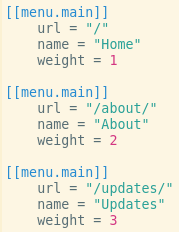
\includegraphics{images/04-newpage_5.png}

\begin{enumerate}
\def\labelenumi{\arabic{enumi}.}
\setcounter{enumi}{5}
\tightlist
\item
  Run the ``website\_preview.R'' script to build and preview the changes
\end{enumerate}

\hypertarget{creating-a-new-update-post}{%
\section{Creating a New Update Post}\label{creating-a-new-update-post}}

Creating a new update post for the website consists of a few steps.

\begin{enumerate}
\def\labelenumi{\arabic{enumi}.}
\tightlist
\item
  Change your working directory to the ``/website/'' directory if you haven't already
\end{enumerate}

\begin{itemize}
\tightlist
\item
  Note: Using the R package `here' makes this even easier
\end{itemize}

\begin{quote}
setwd(here(``website''))

or

setwd(``./website'') \# assumes you are in project root
\end{quote}

\begin{enumerate}
\def\labelenumi{\arabic{enumi}.}
\setcounter{enumi}{1}
\tightlist
\item
  Use the blogdown function ``new\_post'' to generate the new post
\end{enumerate}

\begin{quote}
blogdown::new\_post(``Update Post Title'', subdir = ``updates'')
\end{quote}

\begin{itemize}
\tightlist
\item
  Note: Blogdown is a layer on-top of a static site generator Hugo which uses the ``posts'' directory for all new posts. You have to specify `subdir = ``updates''\,' to get the new posts to appear in the ``updates'' directory; otherwise you will have to move your Markdown post from the ``posts'' directory to the ``updates'' directory.
\end{itemize}

\begin{enumerate}
\def\labelenumi{\arabic{enumi}.}
\setcounter{enumi}{1}
\tightlist
\item
  A new Markdown file will open with your specified title and a template for the post
\end{enumerate}

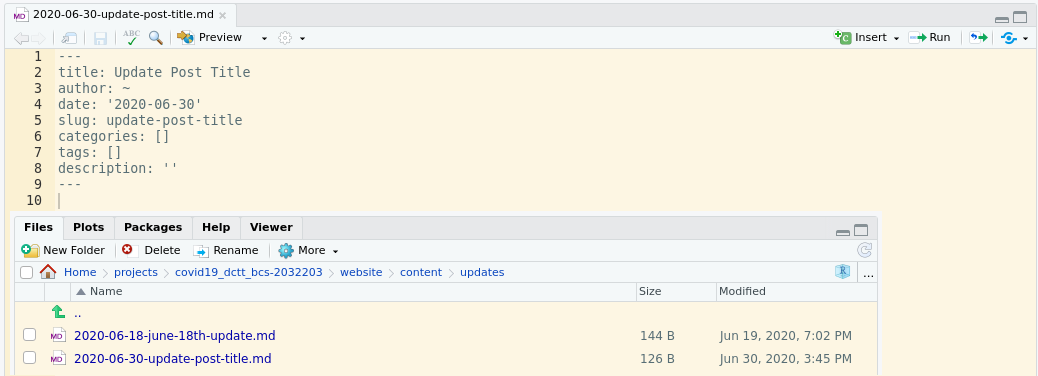
\includegraphics{images/04-newpost_1.png}

\begin{enumerate}
\def\labelenumi{\arabic{enumi}.}
\setcounter{enumi}{2}
\tightlist
\item
  Modify the post file to your liking and run the ``website\_preview.R'' script to preview the changes
\end{enumerate}

\hypertarget{appendix-resources}{%
\chapter*{Appendix \& Resources}\label{appendix-resources}}
\addcontentsline{toc}{chapter}{Appendix \& Resources}

\hypertarget{git}{%
\section*{Git}\label{git}}
\addcontentsline{toc}{section}{Git}

\href{https://git-scm.com/downloads}{Download Git}.

\href{https://git-scm.com/doc}{Additional Git Documentation}.

\hypertarget{markdown}{%
\section*{Markdown}\label{markdown}}
\addcontentsline{toc}{section}{Markdown}

\href{https://www.markdownguide.org/cheat-sheet/}{Markdown Syntax Cheat sheet}

\href{https://www.markdownguide.org/basic-syntax}{Markdown Syntax}

\href{https://www.markdowntutorial.com/lesson/1/}{Markdown Introductory Tutorial}

\hypertarget{r}{%
\section*{R}\label{r}}
\addcontentsline{toc}{section}{R}

\href{https://cloud.r-project.org/}{Download R}.

\hypertarget{rmarkdown}{%
\section*{RMarkdown}\label{rmarkdown}}
\addcontentsline{toc}{section}{RMarkdown}

\href{https://bookdown.org/yihui/rmarkdown/}{RMarkdown Guide}.

\hypertarget{rstudio}{%
\section*{RStudio}\label{rstudio}}
\addcontentsline{toc}{section}{RStudio}

\href{https://rstudio.com/products/rstudio/download/\#download}{Download RStudio}.

\hypertarget{project-source-code}{%
\section*{Project Source Code}\label{project-source-code}}
\addcontentsline{toc}{section}{Project Source Code}

\href{https://github.com/Peter-Kedron/COVID-19-Digital-Contact-Tracing-and-Geospatial-Technologies-and-Privacy}{GitHub}.

  \bibliography{book.bib,packages.bib}

\end{document}
